% !TEX encoding = UTF-8 Unicode
% !TEX TS-program = XeLaTeX
\documentclass[UTF8,12pt,letterpaper,oneside]{amsart}
\usepackage[letterpaper]{geometry}
\geometry{top=1.0in, bottom=1.0in, left=1.0in, right=1.0in}
\usepackage{setspace}
%\doublespacing
\usepackage{hyperref}
%\usepackage{times}
\usepackage{graphicx}
\usepackage{rotating}
\usepackage{multirow}
\usepackage{lineno} 
\usepackage{fancyhdr}
\usepackage{hanging}
\pagestyle{fancy}
\rhead{\textsc{Yang} \thepage} 
\renewcommand{\headrulewidth}{0pt} 
\renewcommand{\footrulewidth}{0pt} 
\setlength\headsep{0.333in}
\usepackage{tikz}
%\usepackage{shapes,backgrounds}

\newenvironment{workscited}{\newpage \begin{center} Works Cited \end{center}}{\newpage }

\begin{document}

\noindent Luke \textsc{Yang}\\
\texttt{1004-3383-46}\\
CSCI 170 MW afternoon lecture\\
\textsc{Professor} Aaron \textsc{Cote}\\
Due Tuesday, January 28, 2014\\
Homework \#1\\

2. 

(a) 

\begin{tikzpicture}

\def\firstcircle{(0,0) circle (1.5cm)}
\def\secondcircle{(55:2cm) circle (1.5cm)}
\def\thirdcircle{(0:2cm) circle (1.5cm)}

\begin{scope}
\fill[gray] \firstcircle;
\end{scope}

\begin{scope}
\clip \firstcircle;
\fill  [white]
\secondcircle;
\end{scope}

\draw \firstcircle node[text=white, below] {$D$};
\draw \secondcircle node [above] {$S$};
\draw \thirdcircle node [below] {$L$};
    
\end{tikzpicture}
Grey area: $D - D \cap S$

(b)

\begin{tikzpicture}

\def\firstcircle{(0,0) circle (1.5cm)}
\def\secondcircle{(55:2cm) circle (1.5cm)}
\def\thirdcircle{(0:2cm) circle (1.5cm)}

\begin{scope}
\fill[gray] \firstcircle;
\fill[gray] \secondcircle;
\end{scope}

\begin{scope}
\clip \secondcircle;
\fill  [white]
\thirdcircle;
\end{scope}

\draw \firstcircle node[text=white, below] {$D$};
\draw \secondcircle node [text=white, above] {$S$};
\draw \thirdcircle node [below] {$L$};
    
\end{tikzpicture}
Grey area: $D \cup S - S \cap L$

(c)

\begin{tikzpicture}

\def\firstcircle{(0,0) circle (1.5cm)}
\def\secondcircle{(55:2cm) circle (1.5cm)}
\def\thirdcircle{(0:2cm) circle (1.5cm)}

\begin{scope}
\fill[gray] \firstcircle;
\fill[black] \secondcircle;
\end{scope}

\begin{scope}
\clip \secondcircle;
\fill  [white]
\thirdcircle;
\end{scope}

\draw \firstcircle node[text=white, below] {$D$};
\draw \secondcircle node [text=white, above] {$S$};
\draw \thirdcircle node [below] {$L$};
\end{tikzpicture}

Gray area: $D - D \cap S$, black area: $S - S \cap L$, apparently, $(D - D \cap S) \cap (S - S \cap L) = \O$, thus, it doesn't matter if the or is an inclusive ``or'' or an exclusive ``or''.

\newpage

(d)

\begin{tikzpicture}

\def\firstcircle{(0,0) circle (1.5cm)}
\def\secondcircle{(55:2cm) circle (1.5cm)}
\def\thirdcircle{(0:2cm) circle (1.5cm)}

\begin{scope}
\fill[gray] \firstcircle;
\fill[gray] \secondcircle;
\end{scope}

\begin{scope}
\clip \secondcircle;
\fill  [white]
\thirdcircle;
\end{scope}

\begin{scope}
\clip \firstcircle;
\fill  [white]
\thirdcircle;
\end{scope}

\draw \firstcircle node[text=white, below] {$D$};
\draw \secondcircle node [text=white, above] {$S$};
\draw \thirdcircle node [below] {$L$};
    
\end{tikzpicture}
fig. 1: Gray area: $|{\overline L}| = |U| - |L|$

\begin{tikzpicture}

\def\firstcircle{(0,0) circle (1.5cm)}
\def\secondcircle{(55:2cm) circle (1.5cm)}
\def\thirdcircle{(0:2cm) circle (1.5cm)}

\begin{scope}
\fill[gray] \firstcircle;
\fill[gray] \thirdcircle;
\end{scope}

\begin{scope}
\clip \secondcircle;
\fill  [white]
\thirdcircle;
\end{scope}

\begin{scope}
\clip \firstcircle;
\fill  [white]
\secondcircle;
\end{scope}

\draw \firstcircle node[text=white, below] {$D$};
\draw \secondcircle node [above] {$S$};
\draw \thirdcircle node [text=white, below] {$L$};
    
\end{tikzpicture}
fig. 2: Gray area: $|{\overline S}|$

\begin{tikzpicture}

\def\firstcircle{(0,0) circle (1.5cm)}
\def\secondcircle{(55:2cm) circle (1.5cm)}
\def\thirdcircle{(0:2cm) circle (1.5cm)}

\begin{scope}
\fill[gray] \firstcircle;
\end{scope}

\begin{scope}
\clip \firstcircle;
\fill  [white]
\thirdcircle;
\end{scope}

\begin{scope}
\clip \firstcircle;
\fill  [white]
\secondcircle;
\end{scope}

\draw \firstcircle node[text=white, below] {$D$};
\draw \secondcircle node [above] {$S$};
\draw \thirdcircle node [below] {$L$};
    
\end{tikzpicture}
fig. 3: (From fig. 1 and fig. 2) gray area: $|{\overline L} \cap {\overline S}|$

\begin{tikzpicture}

\def\firstcircle{(0,0) circle (1.5cm)}
\def\secondcircle{(55:2cm) circle (1.5cm)}
\def\thirdcircle{(0:2cm) circle (1.5cm)}

\begin{scope}
\clip \secondcircle;
\fill  [gray]
\thirdcircle;
\end{scope}

\draw \firstcircle node[below] {$D$};
\draw \secondcircle node [above] {$S$};
\draw \thirdcircle node [below] {$L$};
    
\end{tikzpicture}
fig. 4: Gray area: $|L \cap S|$

\newpage

\begin{tikzpicture}

\def\firstcircle{(0,0) circle (1.5cm)}
\def\secondcircle{(55:2cm) circle (1.5cm)}
\def\thirdcircle{(0:2cm) circle (1.5cm)}

\begin{scope}
\fill[gray] \firstcircle;
\fill[gray] \secondcircle;
\end{scope}

\begin{scope}
\clip \firstcircle;
\fill  [white]
\thirdcircle;
\end{scope}

\begin{scope}
\clip \firstcircle;
\clip \secondcircle;
\fill [gray] \thirdcircle;
\end{scope}

\draw \firstcircle node[text=white, below] {$D$};
\draw \secondcircle node [text=white, above] {$S$};
\draw \thirdcircle node [below] {$L$};
    
\end{tikzpicture}
fig. 5: (From fig. 1 and fig. 4) gray area: $|U| - |L| + |L \cap S|$

\begin{tikzpicture}

\def\firstcircle{(0,0) circle (1.5cm)}
\def\secondcircle{(55:2cm) circle (1.5cm)}
\def\thirdcircle{(0:2cm) circle (1.5cm)}

\begin{scope}
\fill[gray] \firstcircle;
\end{scope}

\begin{scope}
\clip \firstcircle;
\fill  [white]
\thirdcircle;
\end{scope}

\begin{scope}
\clip \firstcircle;
\fill  [white]
\secondcircle;
\end{scope}

\draw \firstcircle node[text=white, below] {$D$};
\draw \secondcircle node [above] {$S$};
\draw \thirdcircle node [below] {$L$};
    
\end{tikzpicture}
fig. 6: (From fig. 5) gray area: $|U| - |L| + |L \cap S| - |S|$

Fig. 6 is identical to fig. 3, thus $|{\overline L} \cap {\overline S}| = |U| - |L| - |S| + |L \cap S|$.

3. 

(a)

$$\sum_{i = 1}^8 C_i = C_1 8^B = \$10\text{ mil} \times 8^B = \$40.96\text{ mil}.$$

(b)

$$C_n = \sum_{i = 1}^{n} C_i - \sum_{i = 1}^{n - 1} C_i  = C_1 n^B - \sum_{i = 1}^{n - 1} C_i.$$

(c)

$$C_n = \sum_{i = 1}^{n} C_i - \sum_{i = 1}^{n - 1} C_i = C_1 n^B - C_1 (n - 1)^B = C_1 \left[ n^B - (n - 1)^B \right].$$

(d)

$$C_8 - C_1 = C_1 \left ( 8^B - 7^B - 1\right ) = -\$6.45\text{ mil}.$$

4. 

(a) 

This function is injective but isn't surjective. 

$\forall x_1 \in \mathbf{O} \forall x_2 \in \mathbf{O}(x_1 \neq x_2 \rightarrow f(x_1) = 4x_1 \neq 4x_2 = f(x_2))$, so it is injective.
However, even numbers that are not multiples of 4 (e.g., 6, 14) cannot be produced from this function, so it isn't surjective.

(b) 

This function isn't injective but is surjective. 

For example, $\left \lfloor \dfrac{7}{2} \right \rfloor = 3 = \left \lfloor \dfrac{6}{2} \right \rfloor$, so it is not injective. On the other hand, note that $f(x) = y \Leftrightarrow \left \lfloor \dfrac{x}{2} \right \rfloor = y \Leftrightarrow x = 2y \text{ or } 2y + 1$. Then $\forall y \in \mathbf{Z} \exists x \in \mathbf{Z} (f(x) = y)$, thus it is surjective.

(c) 

This function is bijective.

This function promises that $x$ and $y = f(x)$ has the same parity. As $\mathbf{E}$ and $\mathbf{O}$ are disjoint sets and $\mathbf{E} \cup \mathbf{O} = \mathbf{Z}$, function $f(x)$ can be seen as the combination of two functions $f_1$ and $f_2$, where $f_1: \mathbf{O} \rightarrow \mathbf{O}, f_1(x) = x + 4$, and $f_2: \mathbf{E} \rightarrow \mathbf{E}, f_2(x) = x + 2$. $f_1$ is injective because $\forall x_1 \in \mathbf{O} \forall x_2 \in \mathbf{O}(x_1 \neq x_2 \rightarrow f_1(x_1) = x_1 + 4 \neq x_2 + 4 = f_1(x_2))$. $f_1$ is surjective because $f_1(x) = y \Leftrightarrow x + 4 = y \Leftrightarrow x = y - 4$, which means $\forall y \in \mathbf{O} \exists x \in \mathbf{O} (f_1(x) = y)$. Thus $f_1$ is bijective. Similarly, $f_2$ is bijective. Consequently, $f$ is bijective.

(d) 

This function is neither injective nor surjective.

$f(3) = 4 = f(-3)$, so this function isn't injective. $f(x) = |x| + 1 \geq 1$ always holds, so natural number 0 can never be produced, and this function isn't surjective.

5.

(a) 

When the fourth circle is introduced into a correct 4-Set Venn Diagram, the new diagram has to represent the intersections of the new set and every existing set. This diagram is incorrect because it fails to do so, e.g., it does not represent the interaction of the green set and the ``unique'' yellow set (of which the members belong to yellow set only). Note that a correct $n$-Set Venn Diagram should have $2^n$ distinctive partitions (this number refers to the cardinality of the set that takes these $n$ sets as members). A correct 3-Set Venn Diagram (of sets $A$, $B$, and $C$, for example) has 8 ($= P(\{A, B, C\}$)) distinct partitions, and a correct 4-Set Venn Diagram should have 16 distinct partitions. This diagram does not have 16 distinct partitions.

(b)

\includegraphics[scale=0.4]{hw1-4venn.pdf}

\newpage

(c)

i. 

\includegraphics[scale=0.4]{hw1-4venn2.pdf}

ii. 

\includegraphics[scale=0.4]{hw1-4venn3.pdf}

(d)

This is not true. While being a member of $B$, an element of the \textit{right hand side} must also be a member of either $A$, or $C$, or $D$; however, a member of the \textit{left hand side} can be unique to $B$, i.e., it can belong to no other set. In this case the \textit{left hand side} set is not a subset of the \textit{right hand side} set.

\end{document}

